\documentclass[UTF8,zihao=-4]{ctexart}
        \usepackage[a4paper,margin=2.35cm]{geometry}
        \usepackage{amsmath,amssymb,amsthm,bm}
        \usepackage{booktabs}
        \usepackage{graphicx}
        \usepackage{caption}
        \usepackage{subcaption}
        \usepackage{float}
        \usepackage{enumitem}
        \graphicspath{{../figures/}{../figures/existing/}}

        \title{ThreeQ 系列能量模型系统研究报告：收敛性、训练机制与 MNIST 实验}
        \author{ThreeQ Research}
        \date{2026-04-19}

        \newtheorem{proposition}{命题}

        \begin{document}
        \maketitle

        \begin{abstract}
        本报告系统整理 ThreeQ 系列能量模型截至当前的理论、实现和实验结论，覆盖基础 ThreeQ、EPThreeQ、DThreeQ、CNNThreeQ/EPCNNThreeQ 及 Dplus 机制诊断。理论部分以固定点推断映射 $T(u;W)$ 的局部 Jacobian 谱半径为核心，给出 $\rho(J)<1$ 下的局部收敛条件、小步训练更新保持稳定裕度的解释，并通过受控线性母模型补充 $\rho(J)>1$ 时的指数发散侧证。实验部分汇总 two moons、MNIST small-budget screen、legacy MNIST reproduction、EPThreeQ 调参、DThreeQ longrun/full-data、输入能量与输出监督审计、Dplus/BP/EP 更新方向诊断以及 CNNThreeQ 结构探索。当前证据表明：EPThreeQ 是最稳定的原始 ThreeQ 改进线，MNIST 10k/2k 上可达约 86.5\% accuracy；DThreeQ 的 EP/CE-nudge 分支可学习，full-data restore-best 达到约 88.0\%，但 final accuracy 存在后期崩塌；Dplus residual-delta 规则尚未呈现 BP-like credit assignment；CNNThreeQ 在结构上自然推广了严格转置对称，但仍缺少充分的可比较多 seed benchmark。
        \end{abstract}

        \section{研究对象与核心问题}

        本项目研究一类基于“对称/双向局部预测 + 截断梯度状态更新”的能量模型。它与标准前馈网络的主要差异在于：网络不是一次前向传播得到输出，而是先在每层状态变量上运行局部推断，使相邻层之间的预测残差下降；训练则根据自由相、受扰相或 residual delta 构造权重更新。这个范式的目标不是完全复制 BP，而是在局部状态动力学中形成可训练、可解释、可推广到对称结构的学习规则。

        当前研究围绕四个问题展开：
        \begin{enumerate}[leftmargin=2em]
        \item ThreeQ inference 什么时候收敛，训练更新什么时候会破坏收敛性；
        \item 基础 ThreeQ 与 EPThreeQ 在 two moons 和 MNIST 上的性能差异来自哪里；
        \item DThreeQ/Dplus 是否提供了比 EP 更合理的局部 credit assignment；
        \item 这类结构能否推广到严格转置共享、卷积/反卷积和更一般的对称能量模型。
        \end{enumerate}

        \section{理论框架：固定点推断与训练稳定性}

        ThreeQ 母模型将全局状态记为 $u\in\mathbb{R}^n$，局部预测映射写作
        \begin{equation}
        T(u;W)=\frac{1}{n-1}Wg(u),
        \end{equation}
        其中 $g$ 是逐元素激活函数。固定点 $u^\star$ 满足
        \begin{equation}
        u^\star=T(u^\star;W).
        \end{equation}
        在固定点附近定义扰动 $\delta=u-u^\star$，局部 Jacobian 为
        \begin{equation}
        J(u^\star,W)=\frac{\partial T}{\partial u}(u^\star,W)
        =\frac{1}{n-1}W\operatorname{diag}(g'(u^\star)).
        \end{equation}

        \begin{proposition}[局部推断稳定性]
        若固定点 $u^\star$ 处满足 $\rho(J(u^\star,W))<1$，则离散固定点迭代 $u^{t+1}=T(u^t;W)$ 的线性化扰动满足 $\delta_{t+1}\approx J\delta_t$，并在局部指数收敛。若存在特征值 $|\lambda|>1$，则沿对应不稳定特征方向的扰动在局部线性化系统中指数增长。
        \end{proposition}

        训练稳定性是上述条件的参数连续性推论。令训练更新为
        \begin{equation}
        W^+=W-\eta \nabla_W E(u^\star(W),W).
        \end{equation}
        若当前点存在稳定裕度 $\rho(J)\le 1-\varepsilon$，且梯度范数有界，则足够小的 $\eta$ 会保持更新后 $\rho(J(W^+))<1$。该命题只保证局部 inference 稳定，不保证表示能力、BP-like 更新方向或长程训练不会离开稳定邻域。

        \section{模型家族}

        \subsection{基础 ThreeQ / Base3Q}

        基础分层 ThreeQ 使用每层状态 $x_i$，并通过相邻层双向预测构造局部 residual。下层到上层使用 forward weights，上层到下层使用 backward weights；状态推断通常使用 hard clipping $\operatorname{clip}(x,0,1)$ 来维持有界性；训练主线包括 free phase 和 weak/clamped phase，并对受扰相 total energy 或局部 residual 求权重更新。对应代码包括 \texttt{Base3Q/}、\texttt{Base3QClampWithLinear/} 以及公共实现 \texttt{threeq\_common/}。

        基础 ThreeQ 的优势是结构清楚、局部性强、容易和固定点收敛证明对应；主要问题是 hard clipping 虽然降低局部谱半径，却容易制造状态饱和和弱梯度，且 detach/局部预测会削弱深层监督信号传播。

        \subsection{EPThreeQ / EPBase3Q}

        EPThreeQ 将权重目标改为自由相与受扰相能量差：
        \begin{equation}
        \Delta W \propto -\nabla_W\frac{E(s_\beta,W)-E(s_0,W)}{\beta}.
        \end{equation}
        该规则比 direct total-energy objective 更接近 Equilibrium Propagation 的局部学习思想。实验上，EPThreeQ 在 two moons minimal suite 和 legacy MNIST reproduction 中都显著优于 direct ThreeQ。它的主要超参风险是 $\beta$ 与 weak steps：扰动太弱时信号不足，扰动过强或步数过多时容易出现 early-best 后回退。

        \subsection{DThreeQ / Dplus}

        DThreeQ 使用 tanh 状态和双向 residual，比较自由相与受扰相 residual 的变化。Dplus 典型目标为
        \begin{equation}
        \mathcal{L}_{D+}=\frac{1}{2}\sum_e\|r_e^\beta-r_e^0\|^2.
        \end{equation}
        其直觉是：监督扰动应该在局部 residual 中留下可学习的方向信号，从而避免直接依赖 EP 能量差。当前结果显示，DThreeQ 的 EP-nudge/CE-nudge 分支可以在 MNIST 上学习，但 Dplus residual-delta 分支与 BP 更新方向不对齐，尚不能作为主训练规则扩大 benchmark。

        \subsection{CNNThreeQ / EPCNNThreeQ}

        CNNThreeQ 将局部双向预测推广到卷积结构：正向边使用 \texttt{conv2d}，反向边使用 \texttt{conv\_transpose2d}，这在结构上自然对应严格转置共享。该方向是从 MLP 对称结构推广到卷积/反卷积能量模型的重要候选，但当前只有 legacy 脚本和小预算 stress screen，缺少独立、多 seed、完整预算的 CNN suite。因此本报告将 CNNThreeQ 作为结构推广证据，而不把它作为当前性能主结论。

        \section{实验流程与数据来源}

        本报告只汇总已完成实验，不重新训练模型。主要实验来源包括：
        \begin{itemize}[leftmargin=2em]
        \item \texttt{AllConnected3QNotTrained} 与受控线性母模型：验证 $\rho<1$ 收敛和 $\rho>1$ 发散；
        \item \texttt{experiments/minimal\_suite}：two moons 上直接 ThreeQ 与 EPThreeQ 的多 seed 可比较实验；
        \item \texttt{experiments/mnist\_suite}：MNIST 小预算压力筛查，包含 BP MLP/CNN、ThreeQ、EPThreeQ、DThreeQ、CNNThreeQ；
        \item \texttt{experiments/mnist\_legacy\_repro} 与 \texttt{mnist\_epthreeq\_tune}：直接调用 legacy 类复现原始 ThreeQ/EPThreeQ；
        \item 多个 \texttt{mnist\_dthreeq} 系列 suite：DThreeQ focused、longrun、objective、activation、prediction、input-supervision 与 full-data 检查；
        \item \texttt{experiments/mechanism\_diagnostic} 与 \texttt{dplus\_fix\_diagnostic}：同一 mini-batch 上比较 Dplus、BP、EP 的更新方向与 one-step loss decrease。
        \end{itemize}

        \section{收敛性与发散性实验}

        \subsection{非线性 legacy 推断}

        图~\ref{fig:legacy-inference} 显示，当 $L_g=5,8,10$ 时，后期 $\rho(J)$ 明显低于 1，推断残差下降到 $10^{-5}$ 或更低；当 $L_g=12$ 时仍低于 1 但收敛显著变慢；当 $L_g=15$ 时最终 $\rho(J)>1$，残差停留在约 $1.7\times10^{-1}$，没有进入固定点收敛区间。

        \begin{figure}[H]
        \centering
        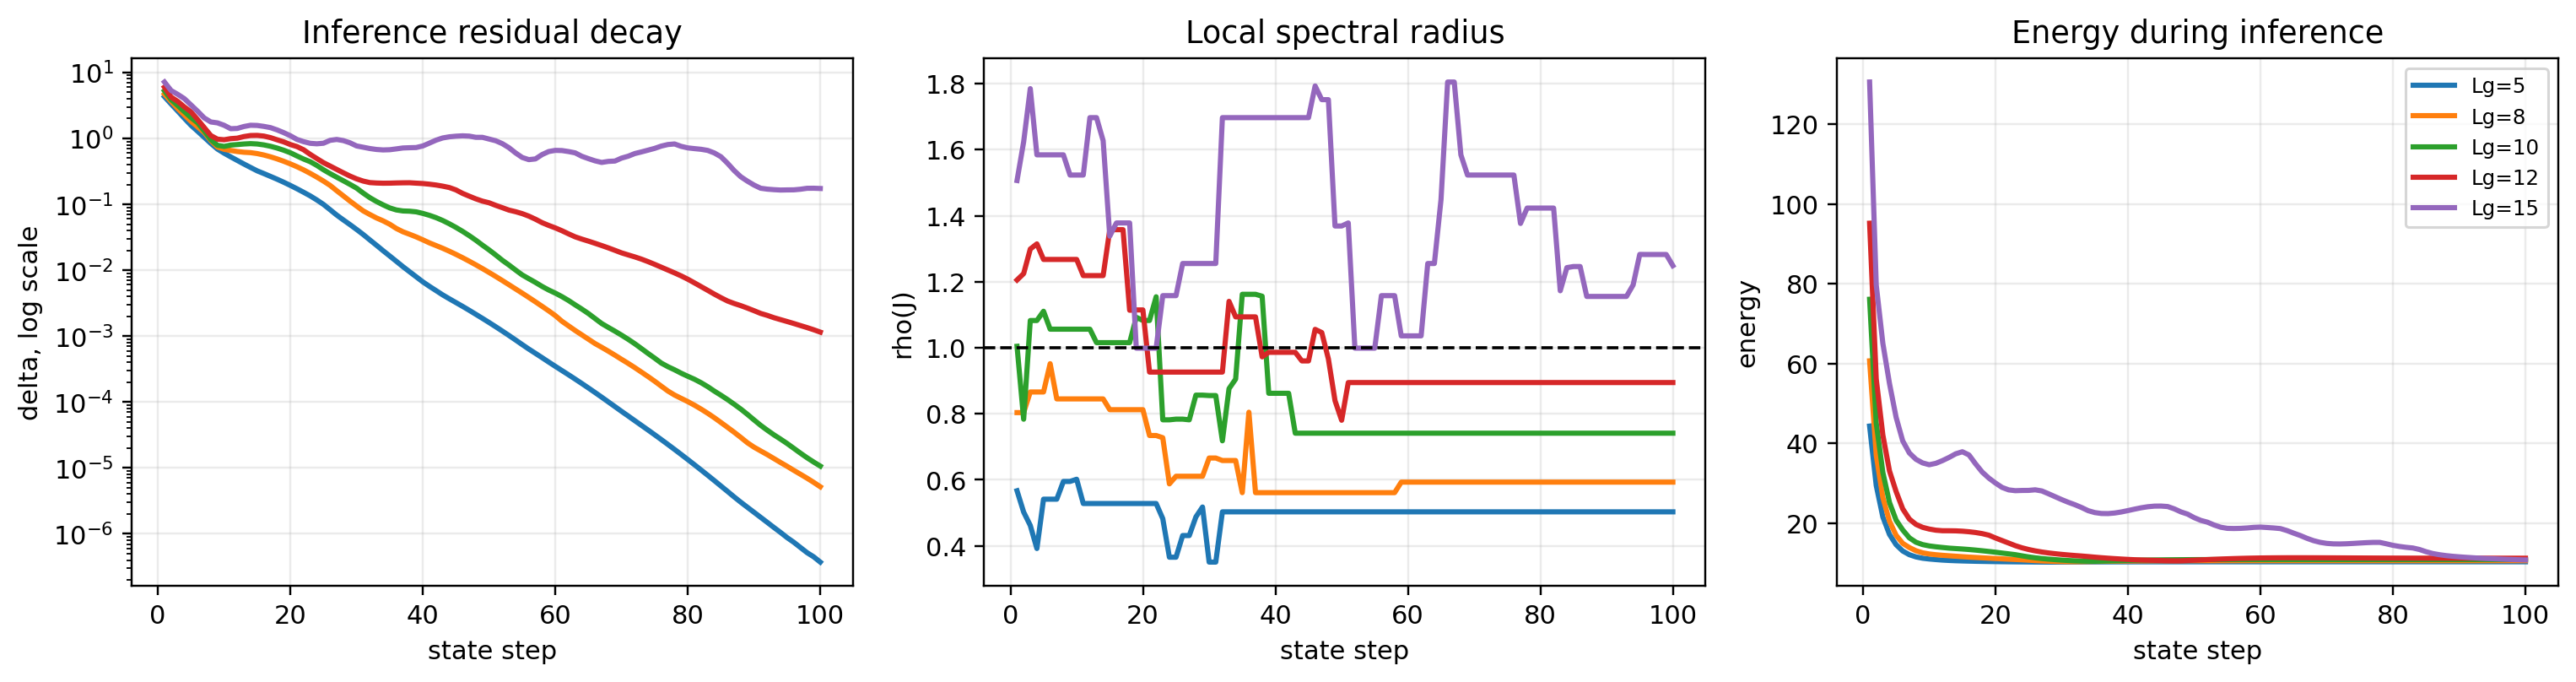
\includegraphics[width=\linewidth]{fig01_threeq_inference_convergence.png}
        \caption{legacy ThreeQ 非线性推断实验。$\rho(J)<1$ 的曲线呈残差衰减；$L_g=15$ 后期 $\rho(J)>1$，表现为非收敛/慢收敛边界。}
        \label{fig:legacy-inference}
        \end{figure}

        \begin{table}[H]
        \centering
        \caption{legacy 推断边界实验摘要。}
        \resizebox{\linewidth}{!}{%
        \begin{tabular}{rrrrrl}
        \toprule
        $L_g$ & initial $\Delta$ & final $\Delta$ & final $\rho$ & reduction & classification \\
        \midrule
        5.0000 & 4.2969 & 3.72e-07 & 0.5029 & 8.66e-08 & convergent \\
8.0000 & 4.7041 & 5.18e-06 & 0.5929 & 1.10e-06 & convergent \\
10.0000 & 5.2755 & 1.07e-05 & 0.7411 & 2.02e-06 & convergent \\
12.0000 & 5.9884 & 0.0012 & 0.8945 & 1.92e-04 & non\_convergent\_or\_slow \\
15.0000 & 7.1753 & 0.1739 & 1.2486 & 0.0242 & non\_convergent\_or\_slow \\
        \bottomrule
        \end{tabular}}
        \end{table}

        \subsection{受控线性推断：$\rho>1$ 的指数发散}

        为了严格隔离谱半径条件，设 $g(u)=u$，并取 $W=(n-1)\rho I$。此时 $T(u;W)=\rho u$，固定点为 $u^\star=0$，且 $J=\rho I$。图~\ref{fig:controlled-inference} 中 $\rho=0.80,0.95$ 时扰动范数下降，$\rho=1.05,1.20$ 时扰动范数指数增长。

        \begin{figure}[H]
        \centering
        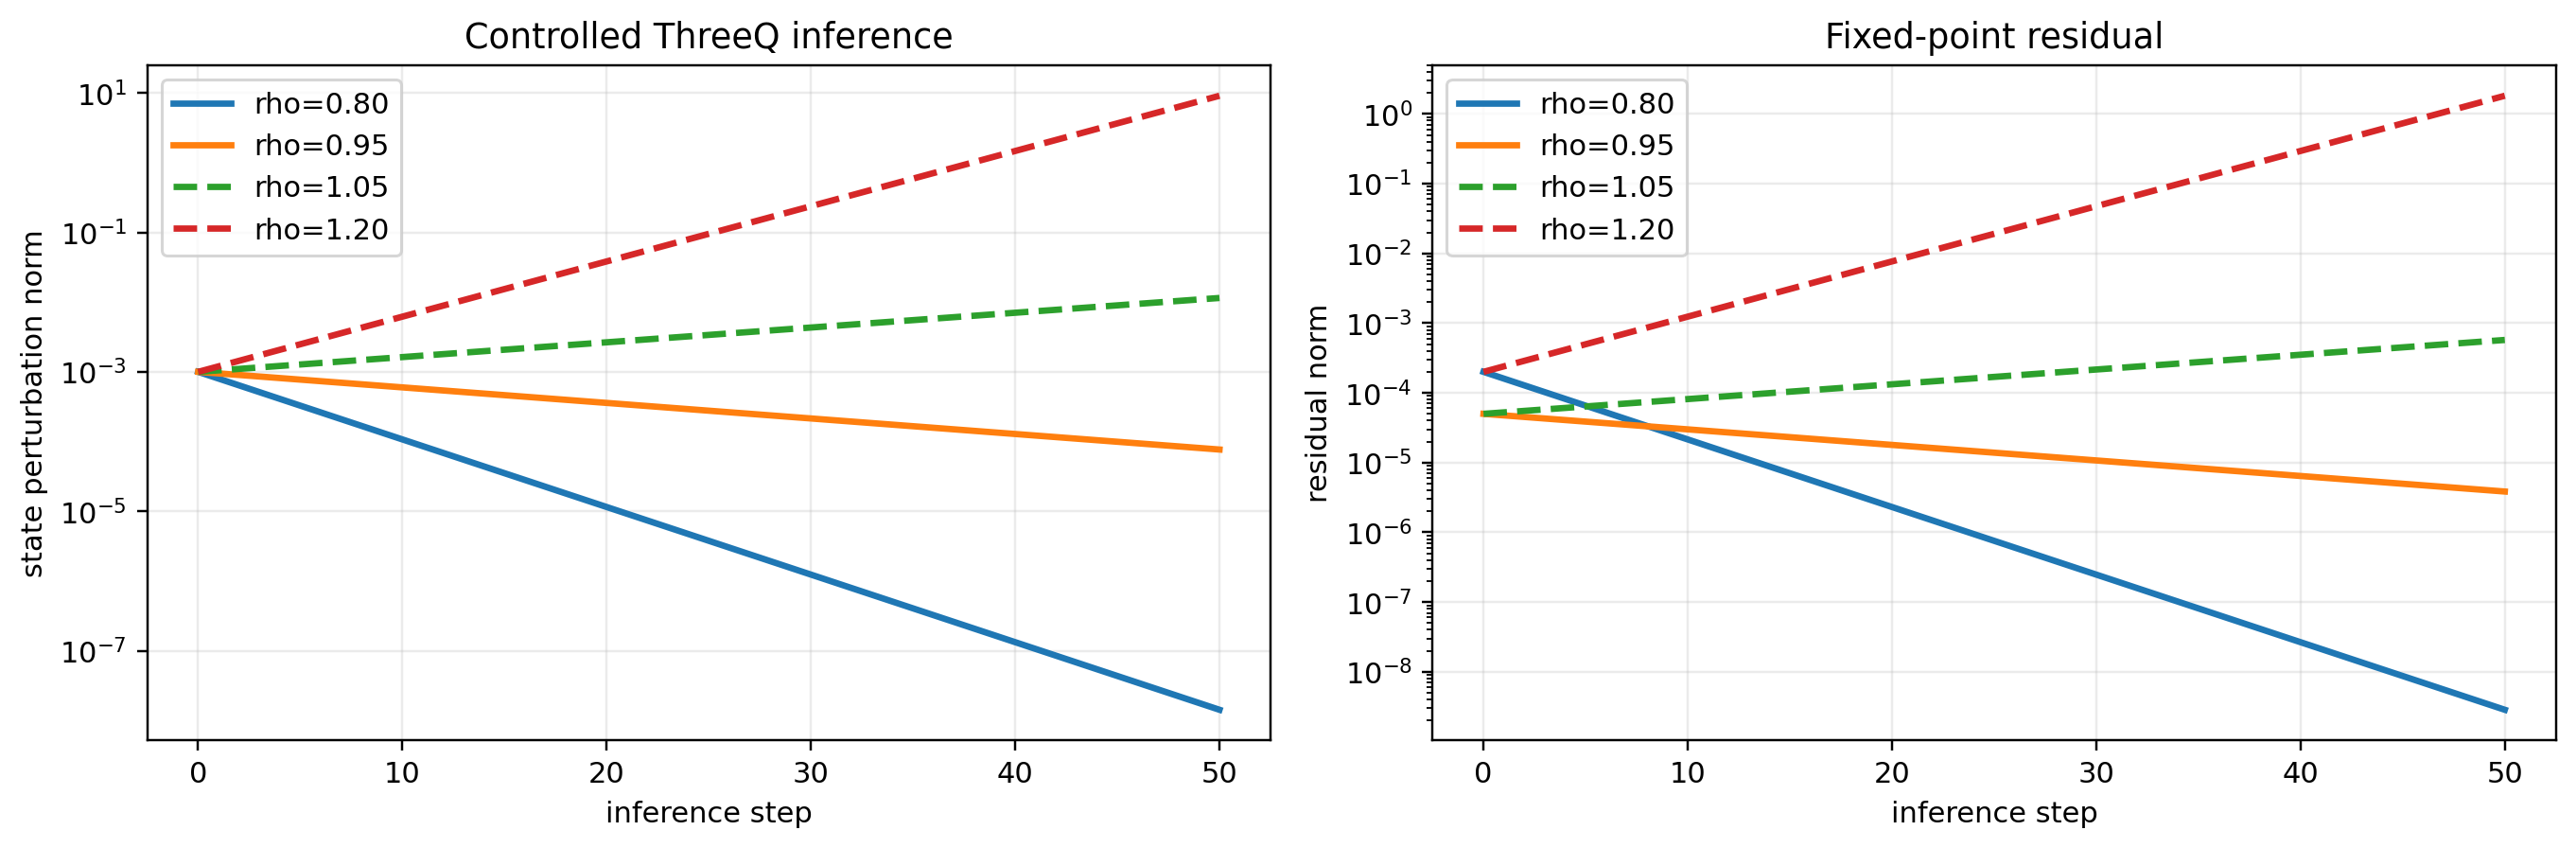
\includegraphics[width=\linewidth]{fig09_controlled_inference_rho_divergence.png}
        \caption{受控线性 ThreeQ 推断实验。在同一固定点更新形式 $u_{t+1}=T(u_t;W)$ 下，$\rho<1$ 收敛，$\rho>1$ 发散。}
        \label{fig:controlled-inference}
        \end{figure}

        \begin{table}[H]
        \centering
        \caption{受控线性推断实验摘要。初始扰动范数为 $10^{-3}$。}
        \resizebox{\linewidth}{!}{%
        \begin{tabular}{lrrrrr}
        \toprule
        case & $\rho$ & initial norm & final norm & growth factor & final residual \\
        \midrule
        stable\_rho\_0p80 & 0.8000 & 0.0010 & 1.43e-08 & 1.43e-05 & 2.85e-09 \\
stable\_rho\_0p95 & 0.9500 & 0.0010 & 7.69e-05 & 0.0769 & 3.85e-06 \\
unstable\_rho\_1p05 & 1.0500 & 0.0010 & 0.0115 & 11.4674 & 5.73e-04 \\
unstable\_rho\_1p20 & 1.2000 & 0.0010 & 9.1004 & 9.10e+03 & 1.8201 \\
        \bottomrule
        \end{tabular}}
        \end{table}

        \subsection{训练更新压力测试}

        图~\ref{fig:training-stress} 展示 bounded-gradient 更新的边界行为。small-step 轨迹从 $\rho=0.70$ 增加到 $0.94$，始终满足 $\rho<1$；large-step 轨迹在第 9 个 epoch 首次达到 $\rho\ge 1$，最终 $\rho=1.54$，最后一轮推断的扰动范数显著增长。

        \begin{figure}[H]
        \centering
        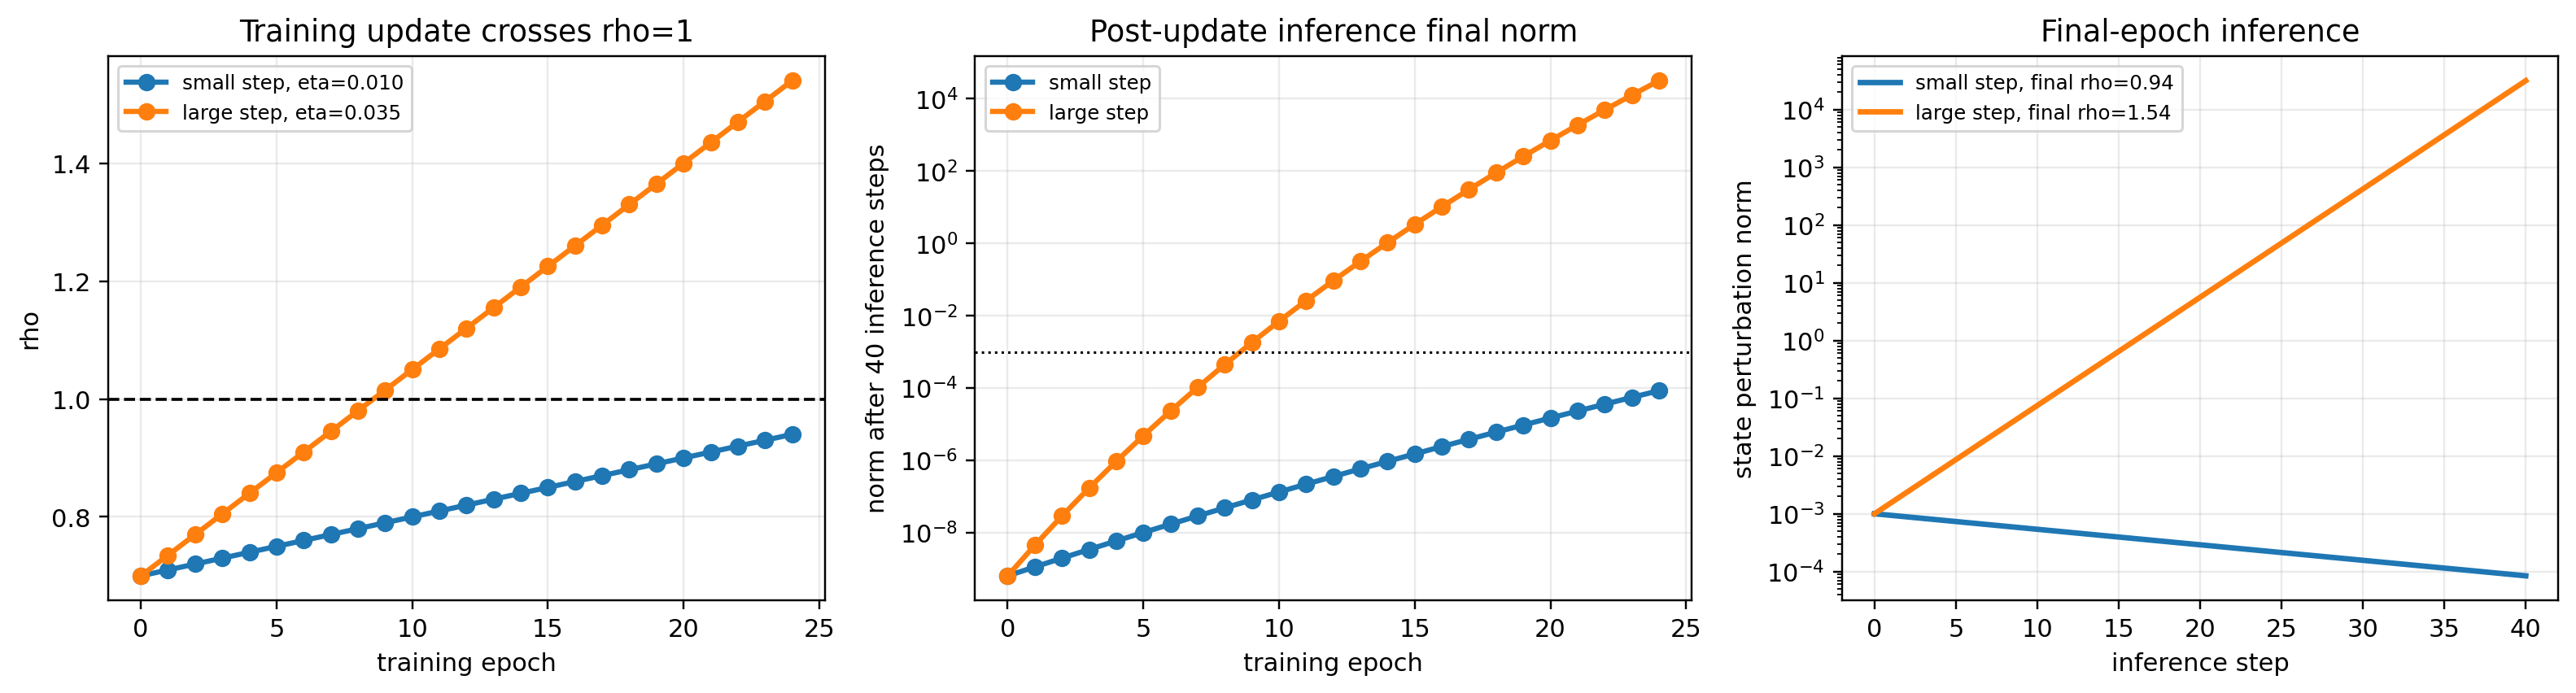
\includegraphics[width=\linewidth]{fig10_training_rho_boundary_stress_test.png}
        \caption{训练更新压力测试。左：训练更新使 $\rho$ 变化；中：每轮更新后推断 40 步的最终扰动范数；右：最后一轮参数下的推断轨迹。}
        \label{fig:training-stress}
        \end{figure}

        \begin{table}[H]
        \centering
        \caption{训练更新压力测试摘要。}
        \resizebox{\linewidth}{!}{%
        \begin{tabular}{lrrrrrr}
        \toprule
        case & $\eta$ & initial $\rho$ & final $\rho$ & first $\rho\ge1$ epoch & growth factor & final norm \\
        \midrule
        small\_step\_eta\_0p010 & 0.0100 & 0.7000 & 0.9400 &  & 0.0842 & 8.42e-05 \\
large\_step\_eta\_0p035 & 0.0350 & 0.7000 & 1.5400 & 9.0000 & 3.17e+07 & 3.17e+04 \\
        \bottomrule
        \end{tabular}}
        \end{table}

        \section{ThreeQ 与 EPThreeQ 实验现象}

        图~\ref{fig:training-convergence} 汇总 legacy ThreeQ/EPThreeQ 的 MNIST 训练曲线。EPBase3Q 在 5k/1k、8 epoch 中达到 77.5\% best validation accuracy，而 Base3Q 为 60.2\%；进一步在 10k/2k、15 epoch 中调参，EPThreeQ 的 best accuracy 达到约 86.5\%。训练中的 \texttt{rho\_mean} 保持在 1 以下，与局部稳定性命题一致。

        \begin{figure}[H]
        \centering
        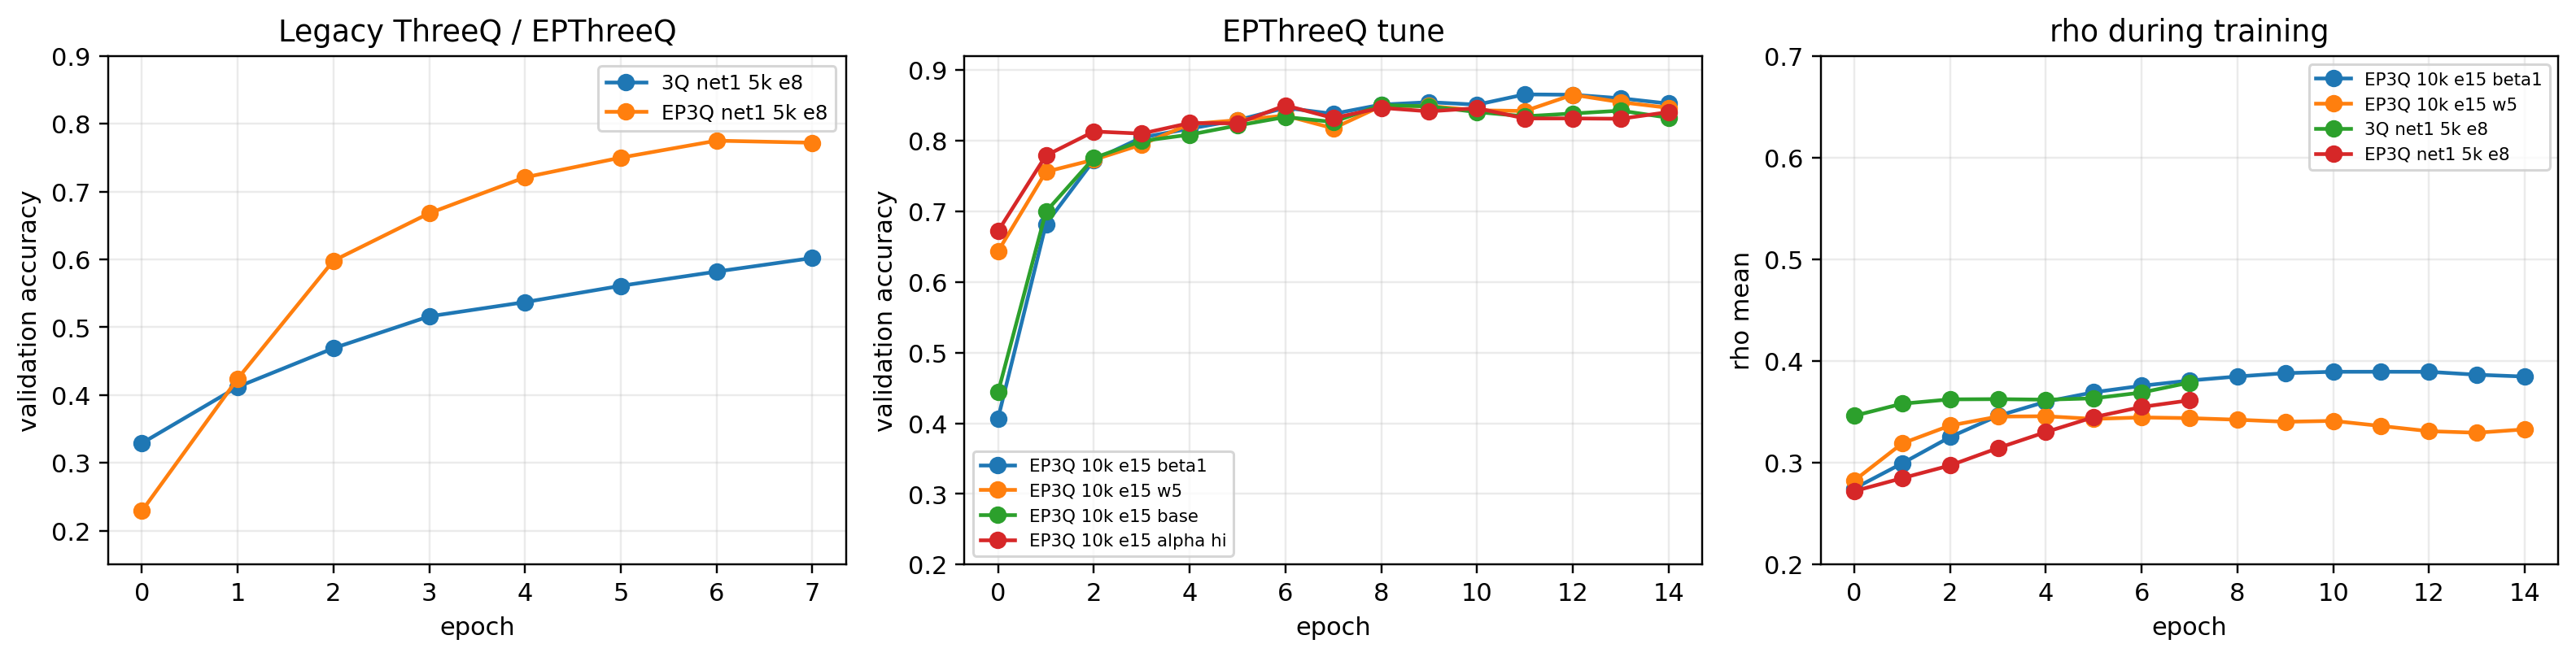
\includegraphics[width=\linewidth]{fig02_threeq_training_convergence.png}
        \caption{legacy ThreeQ/EPThreeQ MNIST 训练曲线与训练过程中的 $\rho$。}
        \label{fig:training-convergence}
        \end{figure}

        \begin{figure}[H]
        \centering
        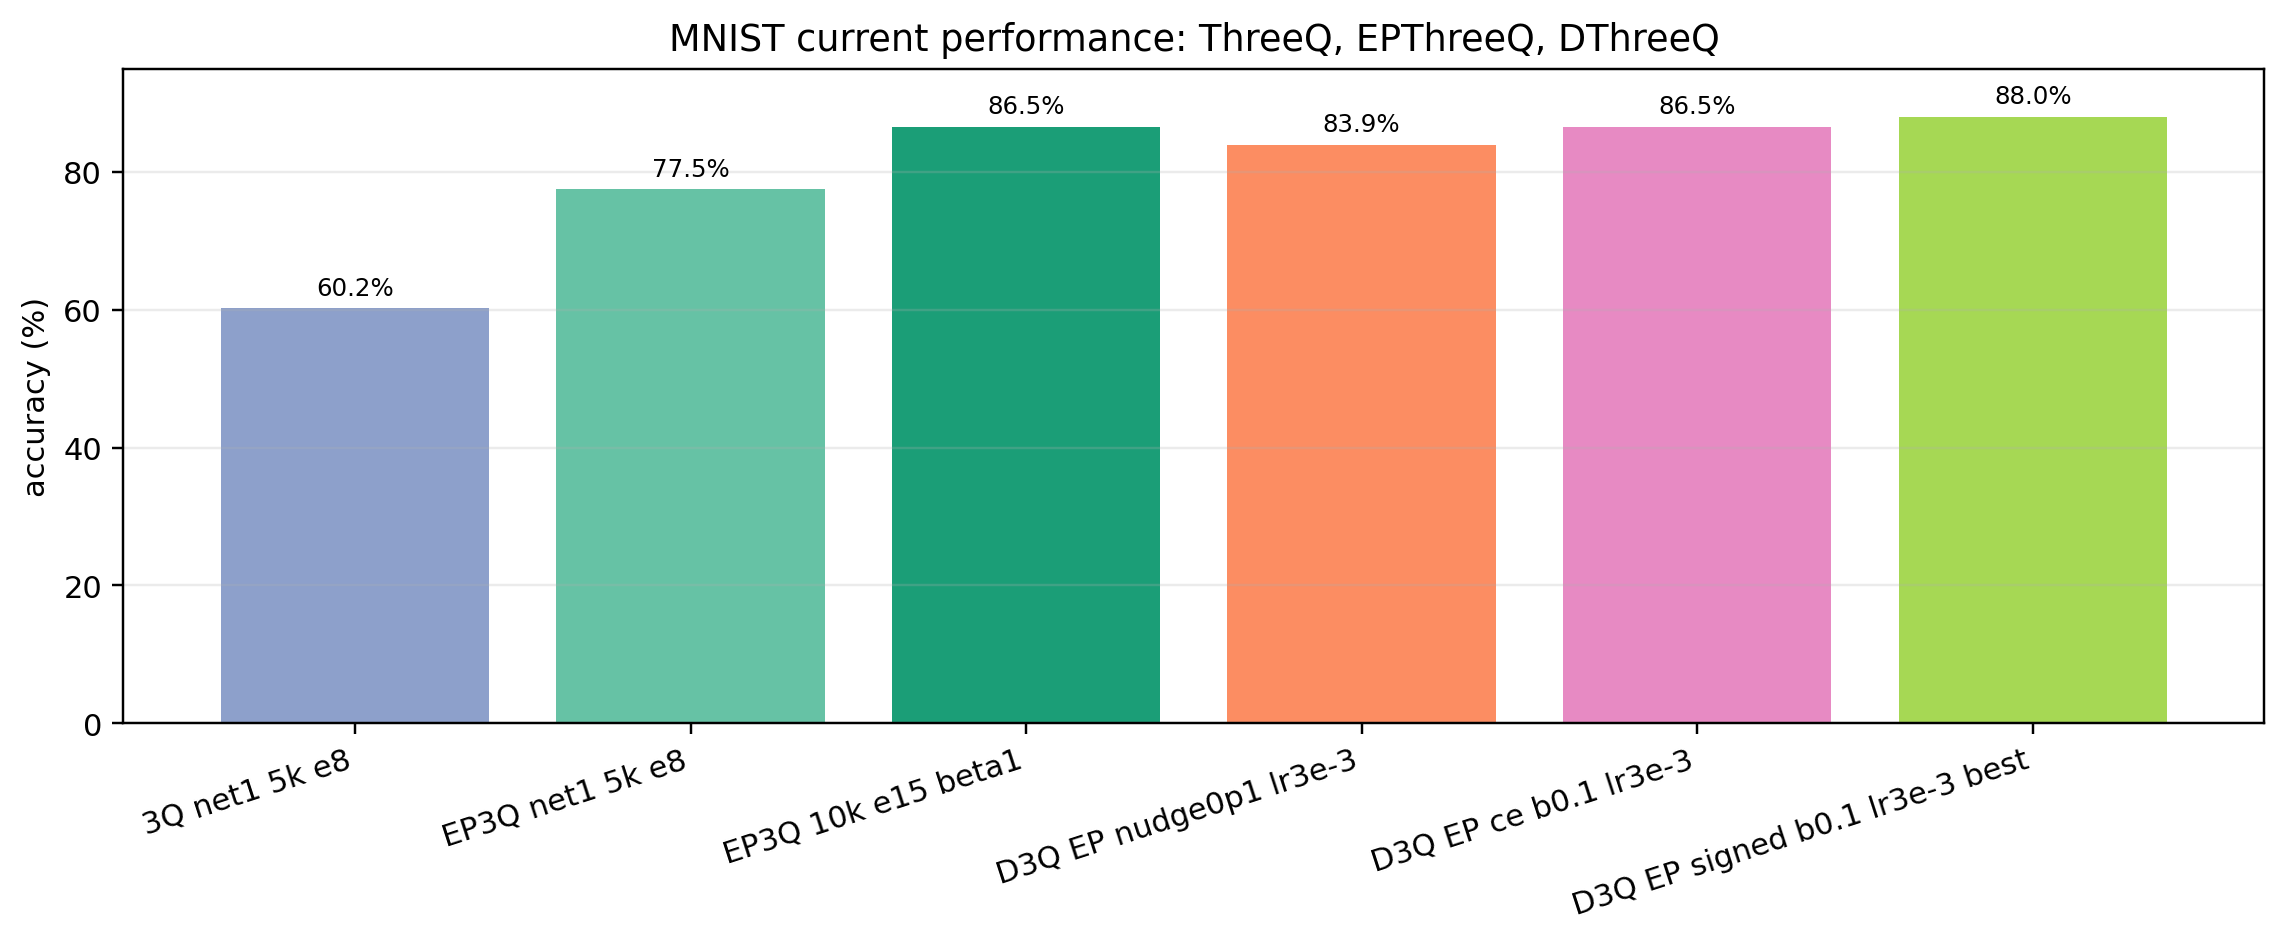
\includegraphics[width=\linewidth]{fig03_mnist_current_performance.png}
        \caption{MNIST 当前性能总览。EPThreeQ legacy 路线和 DThreeQ CE/full-data 路线明显优于小预算公共 ThreeQ screen。}
        \label{fig:mnist-performance}
        \end{figure}

        \begin{table}[H]
        \centering
        \caption{关键性能结果摘录。accuracy\_used 优先使用 selected accuracy，否则使用 best accuracy。}
        \resizebox{\linewidth}{!}{%
        \begin{tabular}{llllrrrr}
        \toprule
        section & dataset & family & variant & best acc. & selected acc. & accuracy used & final error \\
        \midrule
        two\_moons\_minimal & 2D moons, 3 seeds & EPThreeQ & ep\_cost\_w50 & 0.8217 &  & 0.8217 & 0.2817 \\
two\_moons\_minimal & 2D moons, 3 seeds & ThreeQ & direct\_cost\_w10 & 0.6067 &  & 0.6067 & 0.4600 \\
mnist\_epthreeq\_tune & MNIST 10k/2k, 15 epochs & EPThreeQ legacy & epbase3q\_legacy\_10k\_e15\_beta1 & 0.8655 & 0.8655 & 0.8655 & 0.1475 \\
mnist\_dthreeq\_supervision & MNIST 10k/2k, 30 epochs & DThreeQ & dthreeq\_ep\_ce\_nudge0p1\_lr3e3 & 0.8684 & 0.8655 & 0.8655 & 0.1345 \\
mnist\_dthreeq\_supervision & MNIST 10k/2k, 30 epochs & DThreeQ & dthreeq\_ep\_nudge0p1\_lr3e3 & 0.8394 & 0.8354 & 0.8354 & 0.1646 \\
mnist\_dthreeq\_longrun & MNIST 10k/2k, 30 epochs & DThreeQ EP & dthreeq\_ep\_nudge0p1\_lr3e3 & 0.8394 & 0.8394 & 0.8394 & 0.1646 \\
mnist\_legacy\_repro & MNIST 5k/1k, 8 epochs & EPThreeQ legacy & epbase3q\_legacy\_net1\_5k\_e8 & 0.7750 & 0.7750 & 0.7750 & 0.2280 \\
mnist\_legacy\_repro & MNIST 5k/1k, 8 epochs & ThreeQ legacy & base3q\_legacy\_net1\_5k\_e8 & 0.6020 & 0.6020 & 0.6020 & 0.3980 \\
mnist\_dthreeq\_fullbudget & MNIST 60k/10k, 30 epochs & DThreeQ & dthreeq\_ep\_ce\_nudge0p1\_lr3e3 & 0.8790 & 0.8148 & 0.8148 & 0.1852 \\
mnist\_dthreeq\_fullbudget & MNIST 60k/10k, 30 epochs & DThreeQ & dthreeq\_ep\_nudge0p1\_lr3e3 & 0.8523 & 0.1632 & 0.1632 & 0.8368 \\
mnist\_dthreeq\_fullbudget & MNIST 60k/10k, 30 epochs & DThreeQ & dthreeq\_ep\_signed\_nudge0p1\_lr3e3\_restorebest & 0.8803 & 0.8803 & 0.8803 & 0.1621 \\
        \bottomrule
        \end{tabular}}
        \end{table}

        ThreeQ 的主要经验现象是：模型并非不能学习 MNIST，但收敛速度明显慢于 BP，且对 hidden size、状态步数、weak phase、$\beta$ 和训练预算高度敏感。EPThreeQ 相比 direct ThreeQ 更稳定，因为自由相/受扰相差分提供了更明确的局部学习信号。

        \section{DThreeQ 改进过程与当前瓶颈}

        图~\ref{fig:dthreeq-progress} 和图~\ref{fig:dthreeq-curves} 展示 DThreeQ 从 small-budget 失败到 full-data restore-best 约 88.0\% 的改进路径。小预算公共框架下 DThreeQ 接近随机；扩大到 legacy 尺度后，EP-nudge 可到约 80.4\%；30 epoch longrun 到约 83.9\%；CE-style output nudge 在 10k/2k 上达到约 86.5\%；full-data restore-best 达到约 88.0\%，但 final accuracy 明显回退。

        \begin{figure}[H]
        \centering
        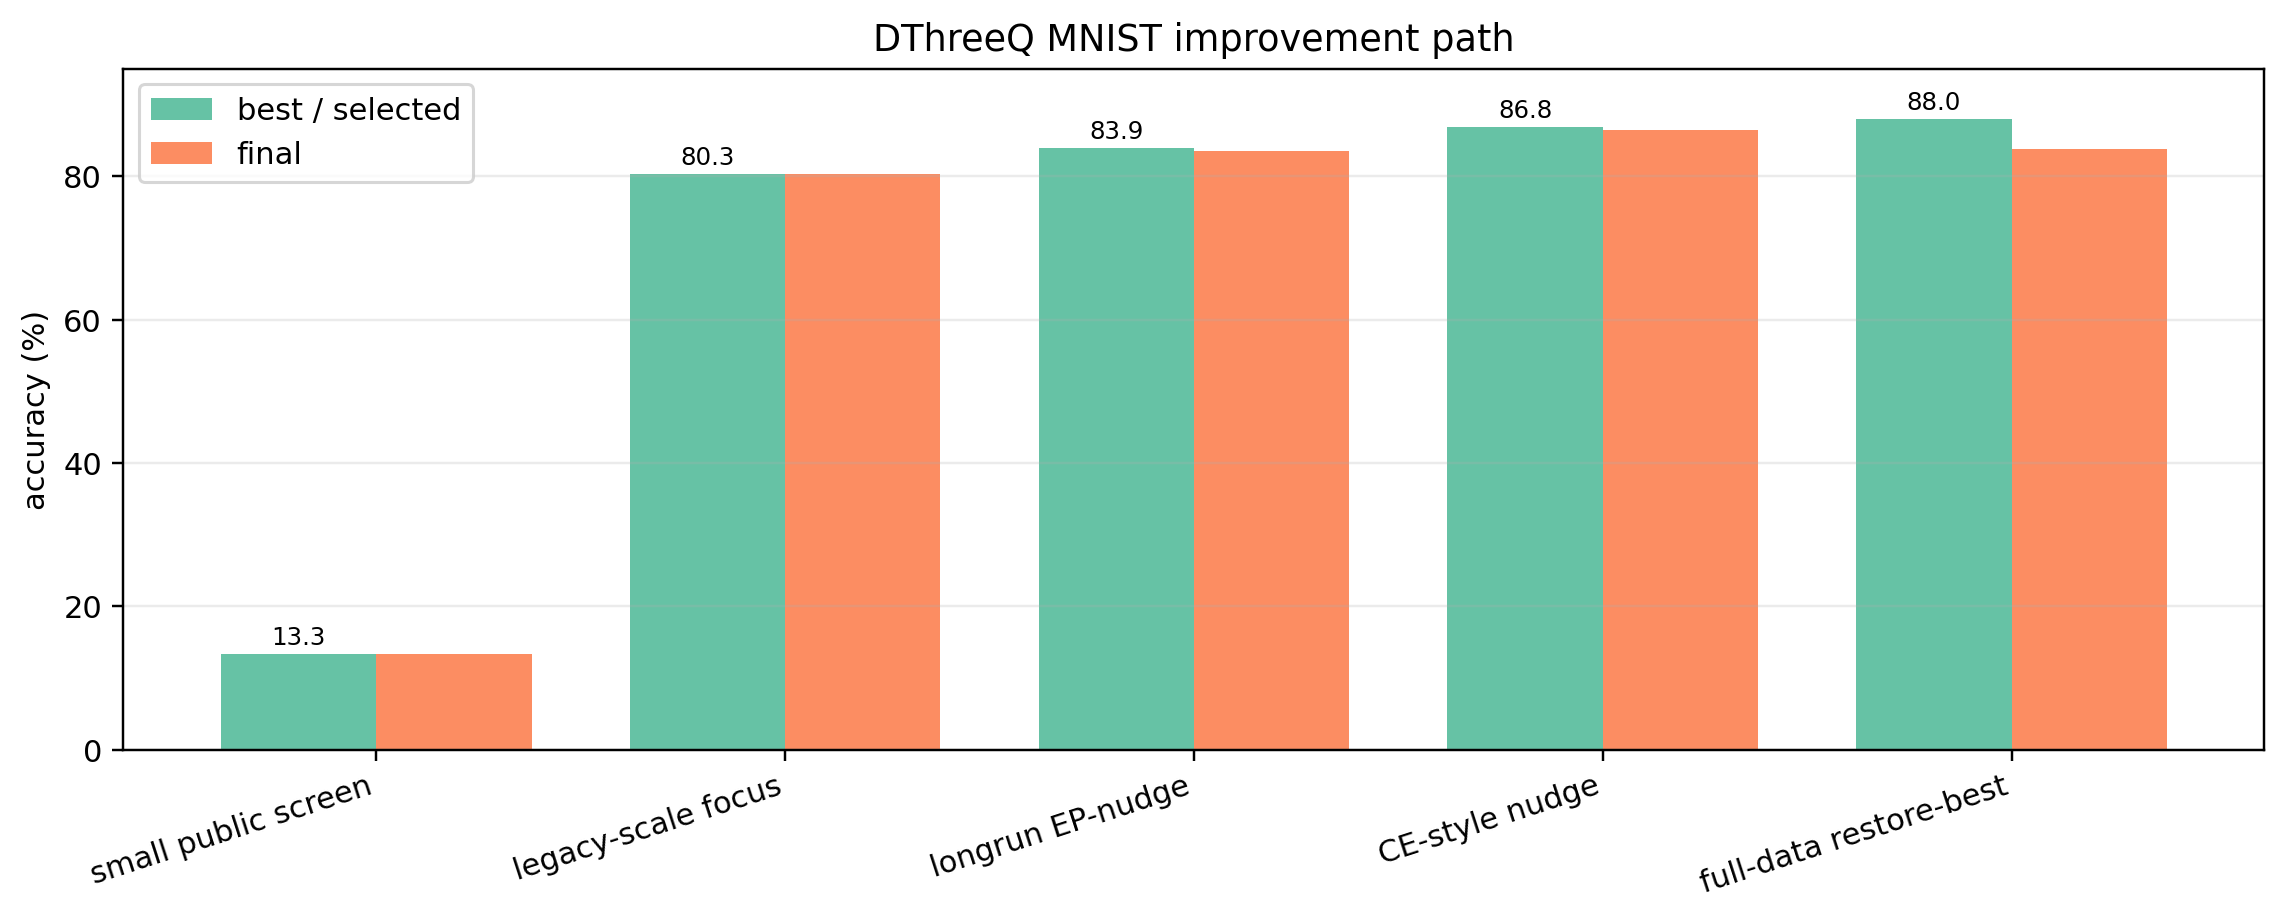
\includegraphics[width=\linewidth]{fig04_dthreeq_improvement_process.png}
        \caption{DThreeQ 从小预算失败到 full-data restore-best 的改进过程。}
        \label{fig:dthreeq-progress}
        \end{figure}

        \begin{figure}[H]
        \centering
        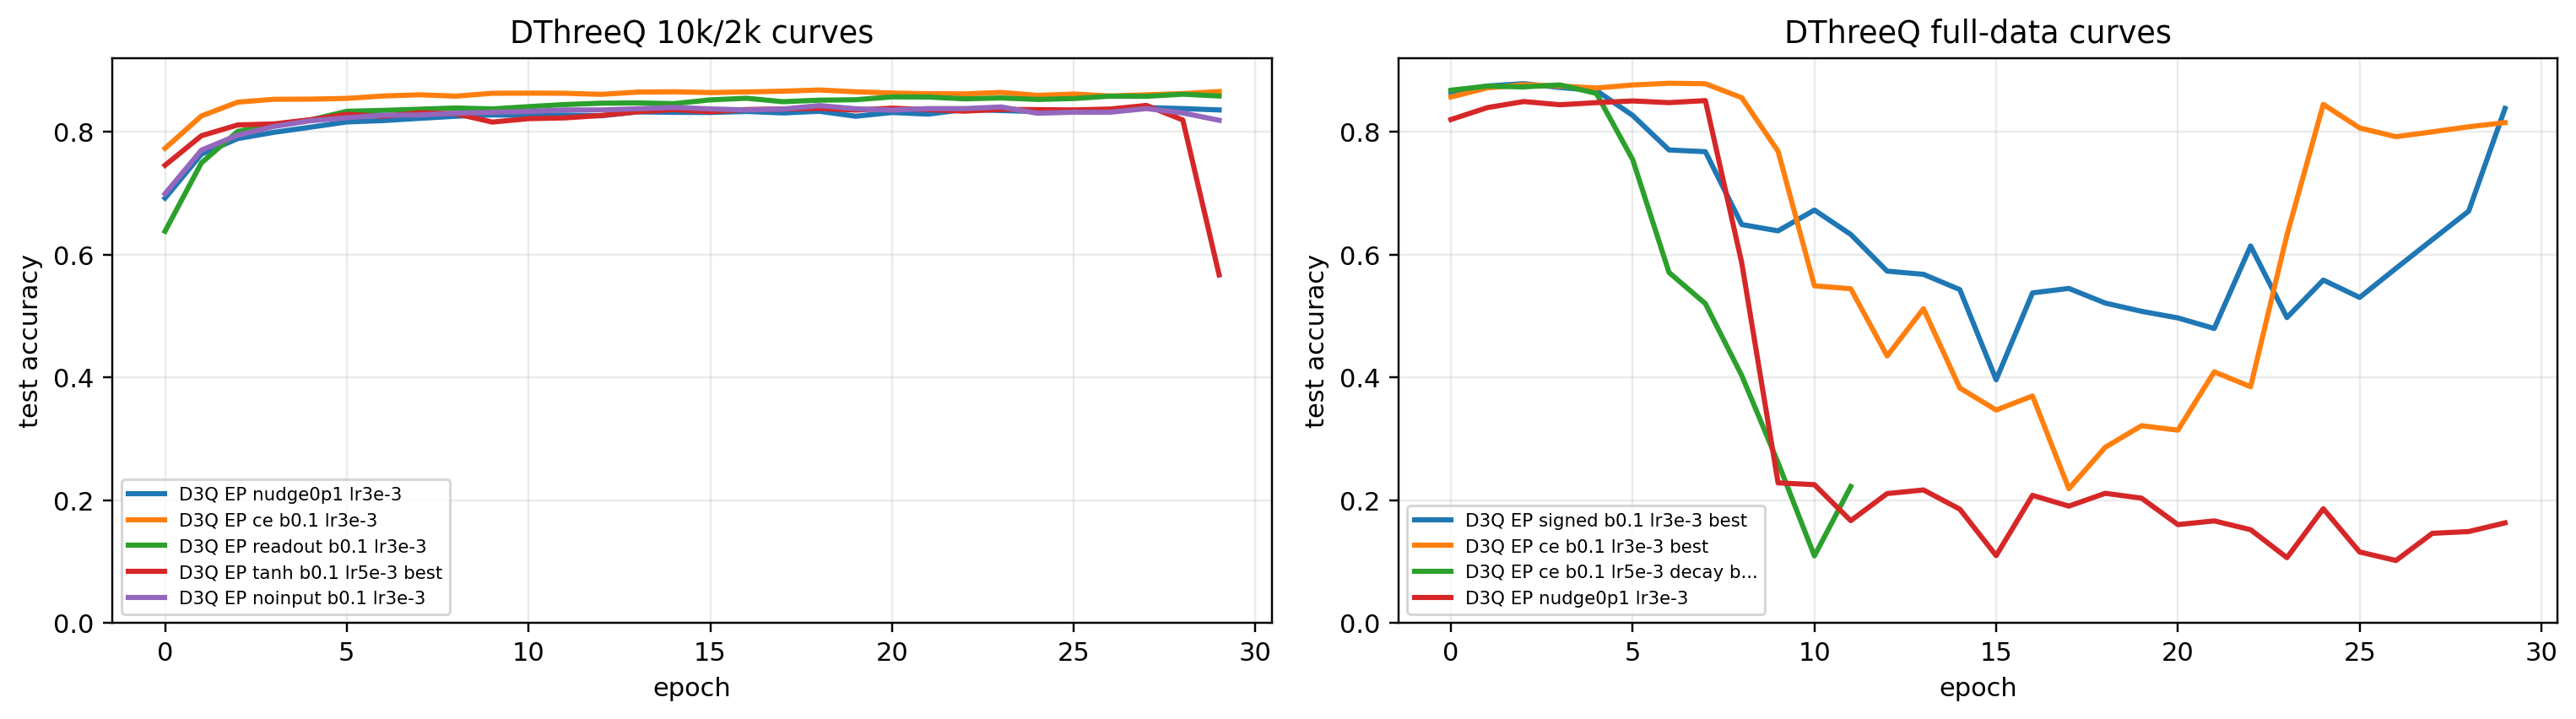
\includegraphics[width=\linewidth]{fig05_dthreeq_training_curves.png}
        \caption{DThreeQ 10k 与 full-data 训练曲线，显示 early-best 与后期崩塌现象。}
        \label{fig:dthreeq-curves}
        \end{figure}

        \begin{table}[H]
        \centering
        \caption{DThreeQ 改进过程分阶段摘要。}
        \resizebox{\linewidth}{!}{%
        \begin{tabular}{lllrrl}
        \toprule
        stage & variant & dataset & best acc. & final acc. & interpretation \\
        \midrule
        small public screen & dthreeq\_ep\_nudge\_0p01 & 3k/1k, 3 epochs & 0.1332 & 0.1332 & 公共框架小预算接近随机，不能代表原始设定。 \\
legacy-scale focus & dthreeq\_ep\_nudge0p1\_lr1e3 & 10k/2k, 12 epochs & 0.8035 & 0.8035 & 放大 hidden size 与训练预算后离开随机。 \\
longrun EP-nudge & dthreeq\_ep\_nudge0p1\_lr3e3 & 10k/2k, 30 epochs & 0.8394 & 0.8354 & 稳定 baseline 约 83.5\% 到 83.9\%。 \\
CE-style nudge & dthreeq\_ep\_ce\_nudge0p1\_lr3e3 & 10k/2k, 30 epochs & 0.8684 & 0.8655 & 输出监督从 MSE nudge 改为 CE-style 后到约 86.5\%。 \\
full-data restore-best & dthreeq\_ep\_signed\_nudge0p1\_lr3e3\_restorebest & 60k/10k, 30 epochs & 0.8803 & 0.8379 & best checkpoint 达 88.0\%，但 final 仍回退。 \\
        \bottomrule
        \end{tabular}}
        \end{table}

        当前 DThreeQ 的结论需要分开表述：EP/CE-nudge 分支已经是可行路线，但 Dplus residual-delta 规则还不能解释外部 90\%+ 结果。若外部 DThreeQ 能稳定超过 90\%，最可能差异来自 CE/softmax 输出、best checkpoint、完整数据预算、额外 readout/pretraining、layer-normalized energy 或更强的后期稳定化。

        \section{Dplus/BP/EP 机制诊断}

        机制诊断在同一 mini-batch 和同一初始参数上比较 Dplus、BP、EP 的更新向量，统计 cosine similarity、norm ratio、sign agreement 和 one-step loss decrease。图~\ref{fig:mechanism-direction} 与图~\ref{fig:mechanism-loss} 显示：Dplus 与 BP 的 forward cosine 只有约 0.03 到 0.08，sign agreement 接近随机；Dplus 与 EP 在 one-sided plus target 上高度同向，但 norm ratio 极小；plusminus 变体出现明确方向抵消。

        \begin{figure}[H]
        \centering
        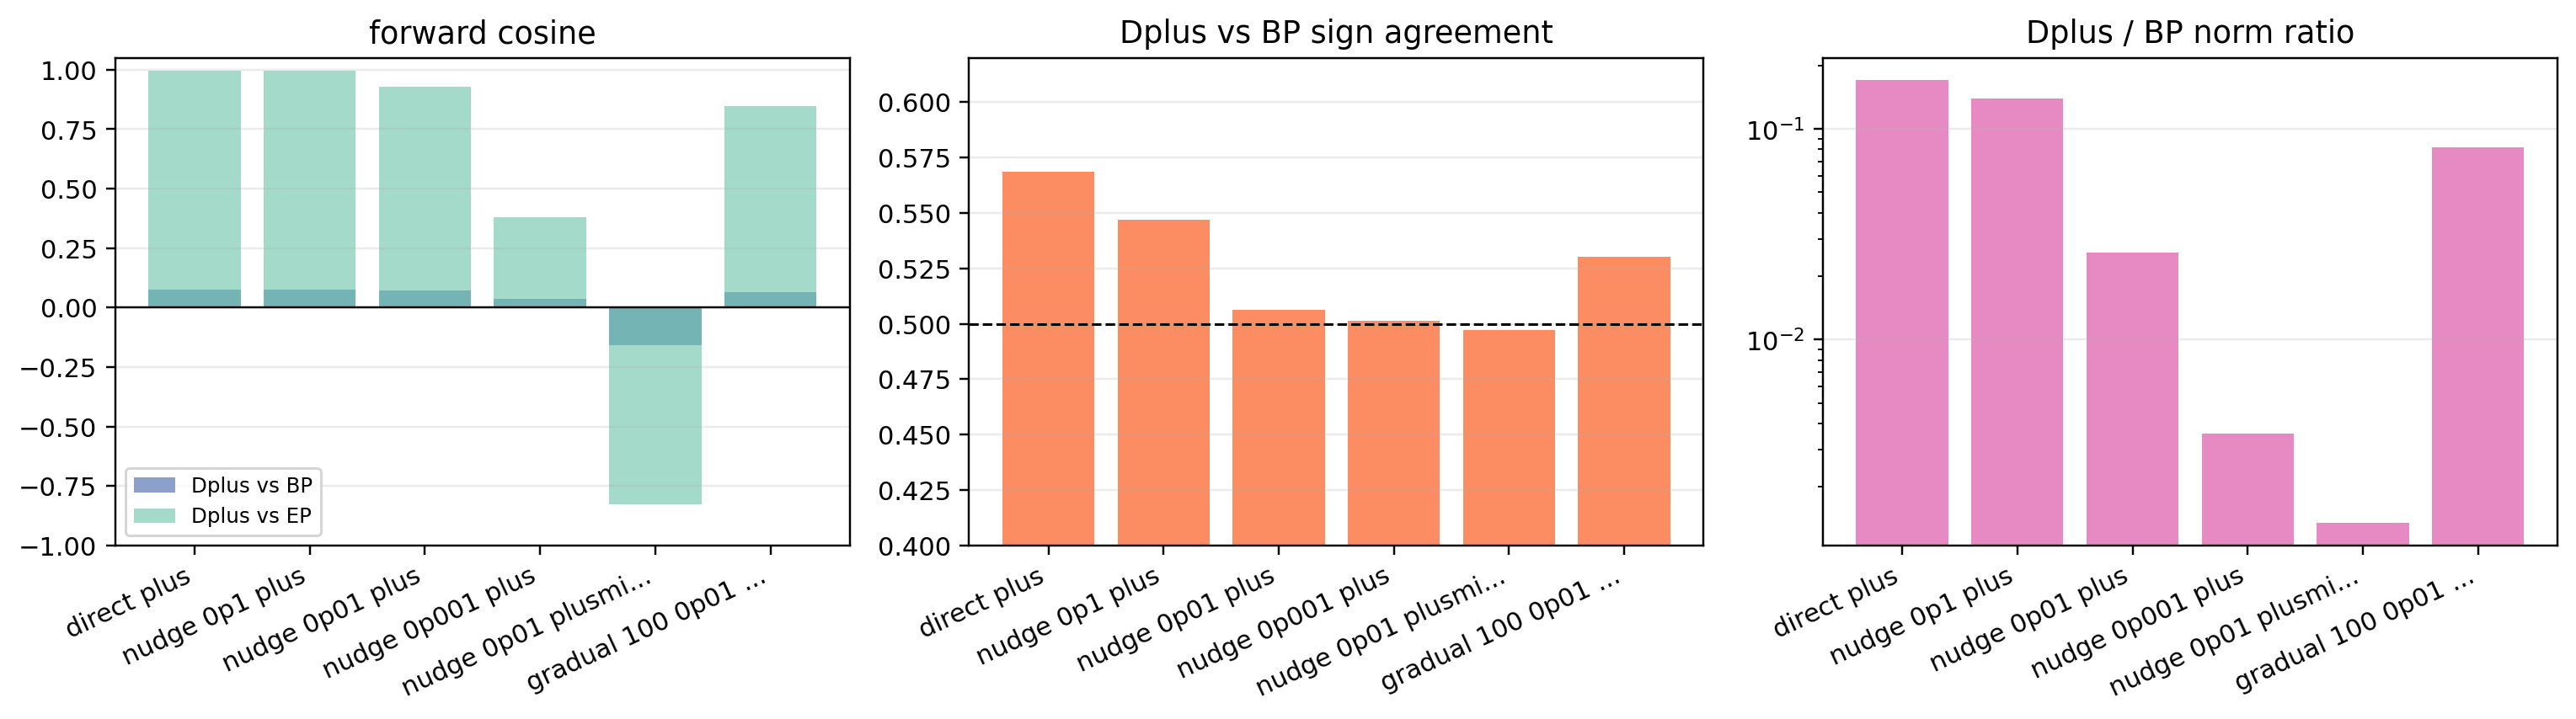
\includegraphics[width=\linewidth]{fig06_mechanism_direction_metrics.png}
        \caption{Dplus、BP、EP 更新向量方向诊断。}
        \label{fig:mechanism-direction}
        \end{figure}

        \begin{figure}[H]
        \centering
        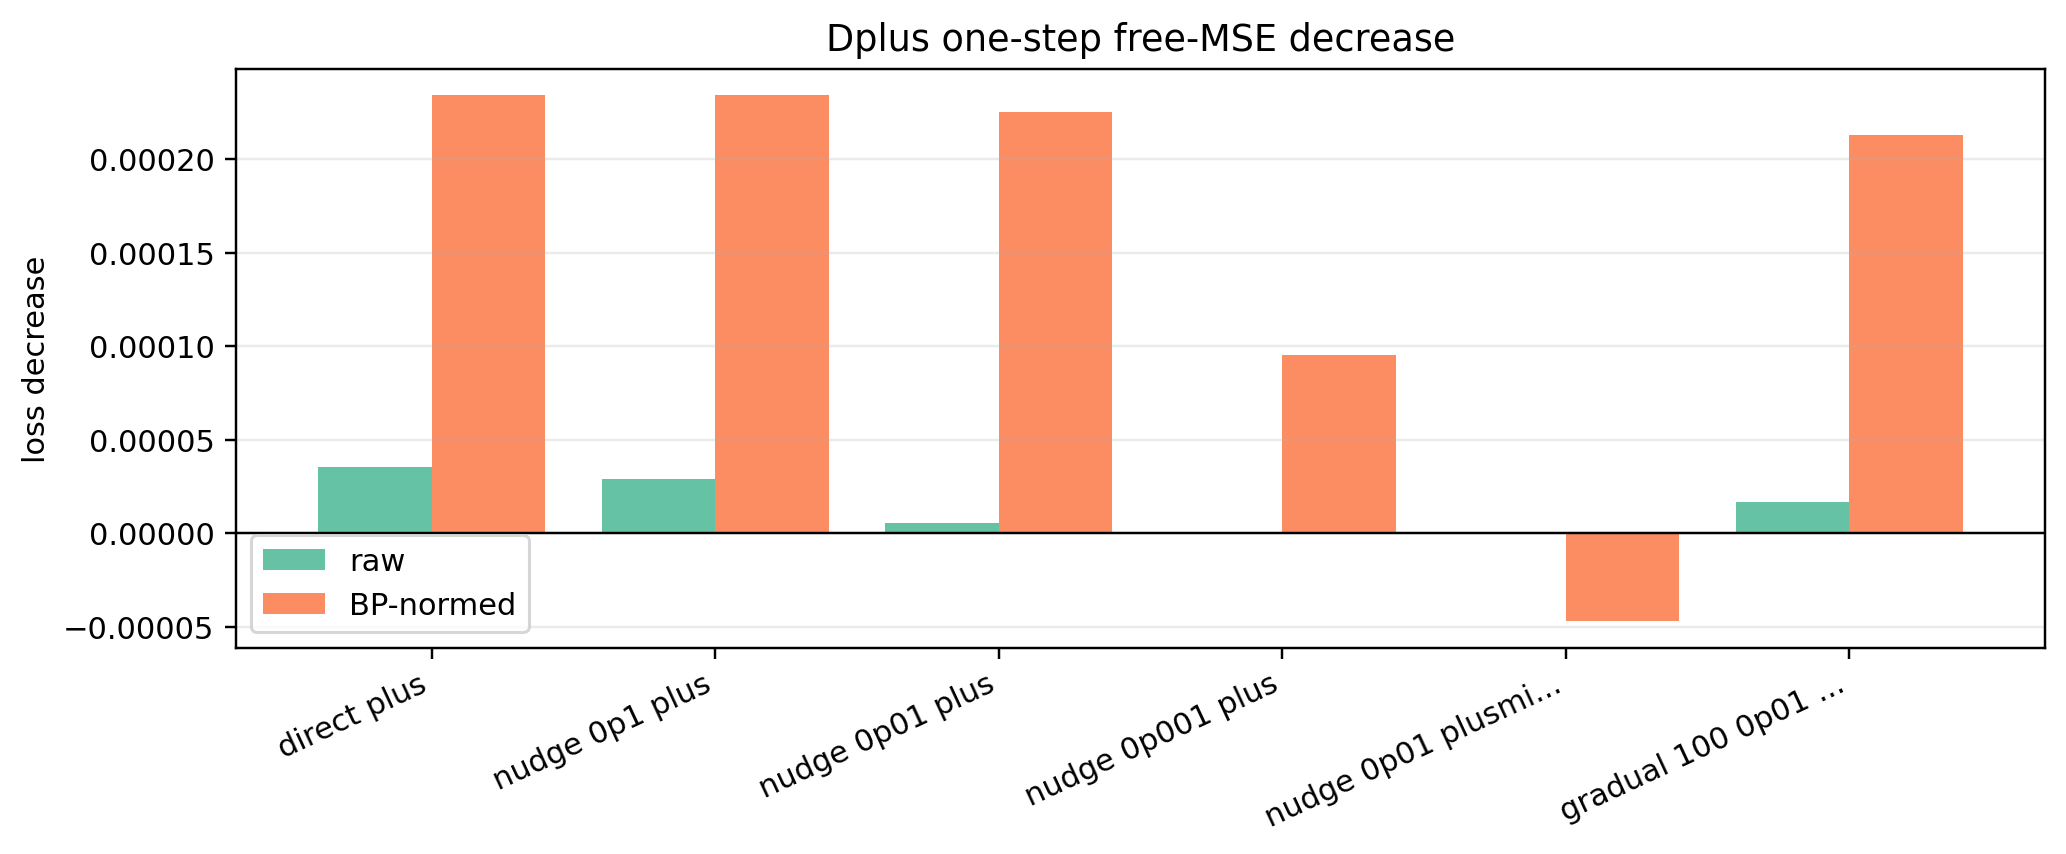
\includegraphics[width=\linewidth]{fig07_mechanism_one_step_loss.png}
        \caption{Dplus one-step loss decrease 与 plusminus 失败模式。}
        \label{fig:mechanism-loss}
        \end{figure}

        \begin{table}[H]
        \centering
        \caption{Dplus 机制诊断关键指标。}
        \resizebox{\linewidth}{!}{%
        \begin{tabular}{lrrrrrr}
        \toprule
        target & BP cosine & BP norm ratio & BP sign & EP cosine & EP norm ratio & raw free-MSE decrease \\
        \midrule
        direct\_plus & 0.0760 & 0.1705 & 0.5685 & 0.9971 & 0.0831 & 3.57e-05 \\
nudge\_0p1\_plus & 0.0750 & 0.1393 & 0.5468 & 0.9967 & 0.0083 & 2.92e-05 \\
nudge\_0p01\_plus & 0.0711 & 0.0259 & 0.5064 & 0.9276 & 7.70e-04 & 5.37e-06 \\
nudge\_0p001\_plus & 0.0363 & 0.0036 & 0.5013 & 0.3804 & 2.55e-05 & 6.73e-07 \\
nudge\_0p01\_plusminus & -0.1574 & 0.0013 & 0.4973 & -0.8290 & 4.62e-05 & -2.96e-07 \\
gradual\_100\_0p01\_plus & 0.0642 & 0.0817 & 0.5303 & 0.8466 & 6.99e-04 & 1.67e-05 \\
        \bottomrule
        \end{tabular}}
        \end{table}

        \begin{table}[H]
        \centering
        \caption{Dplus 修正诊断候选。Residual normalization、scale calibration 和 layer-wise gain 主要改变尺度，尚未改变 BP-like 方向。}
        \resizebox{\linewidth}{!}{%
        \begin{tabular}{llrrrrr}
        \toprule
        objective & target & BP cosine & BP sign & BP norm ratio & EP cosine & BP-scaled free-MSE decrease \\
        \midrule
        resnorm\_layergain\_beta\_div1 & direct\_plus & 0.0762 & 0.5685 & 7.62e+03 & 0.9975 & 4.27e-04 \\
layergain\_beta\_div1 & direct\_plus & 0.0761 & 0.5685 & 0.1705 & 0.9973 & 4.28e-04 \\
resnorm\_beta\_div1 & direct\_plus & 0.0760 & 0.5685 & 7.62e+03 & 0.9972 & 4.27e-04 \\
resnorm\_beta\_div2 & direct\_plus & 0.0760 & 0.5685 & 7.62e+03 & 0.9972 & 4.27e-04 \\
raw & direct\_plus & 0.0760 & 0.5685 & 0.1705 & 0.9971 & 4.27e-04 \\
beta\_div1 & direct\_plus & 0.0760 & 0.5685 & 0.1705 & 0.9971 & 4.27e-04 \\
beta\_div2 & direct\_plus & 0.0760 & 0.5685 & 0.1705 & 0.9971 & 4.27e-04 \\
resnorm\_layergain\_beta\_div1 & nudge\_0p1\_plus & 0.0752 & 0.5468 & 6.23e+04 & 0.9972 & 4.27e-04 \\
        \bottomrule
        \end{tabular}}
        \end{table}

        \section{输入能量、输出监督与后期崩塌}

        图~\ref{fig:input-energy} 汇总 input reconstruction energy 与分类监督的关系。结果显示，输入重构项确实占据较大能量比例，但简单移除或按 $1/784$ 缩放并不能提升 accuracy，反而降低最终表现。这说明输入项既可能压制监督，也在维持表示结构。更合理的方向是 boundary-clamped input、per-layer normalized energy、output CE nudge 和保守 learning-rate schedule。

        \begin{figure}[H]
        \centering
        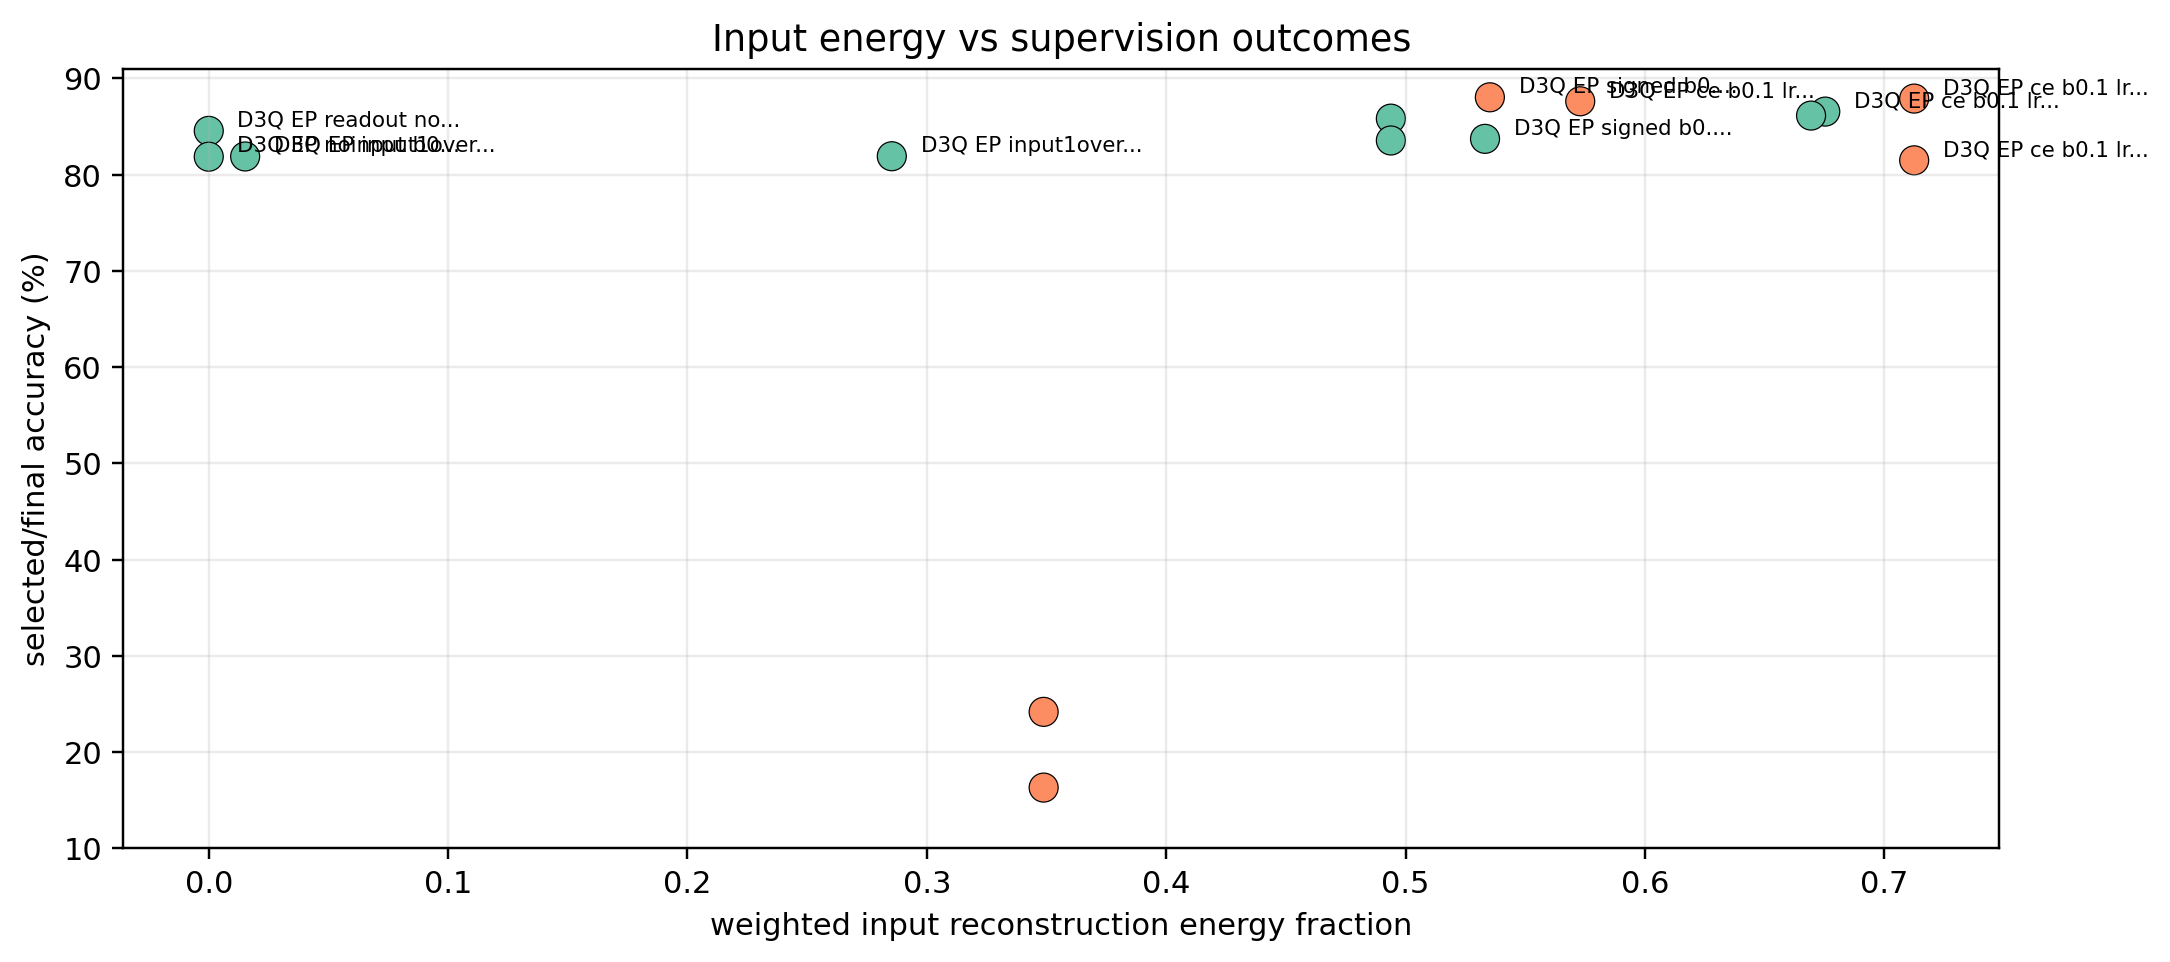
\includegraphics[width=\linewidth]{fig08_input_energy_supervision.png}
        \caption{输入重构能量比例与分类 accuracy 的关系。}
        \label{fig:input-energy}
        \end{figure}

        CE-style output nudge 是当前最明确的正向改动：10k/2k 上把 DThreeQ selected accuracy 提高到约 86.5\%，full-data restore-best 可达约 87.9\%。但 full-data final accuracy 仍会退化，说明仅改监督形式不足以解决后期 saturation、weight drift 或状态轨迹漂移。

        \section{CNNThreeQ 与对称结构推广}

        CNNThreeQ/EPCNNThreeQ 使用卷积/反卷积作为局部双向预测，是严格对称结构的重要推广。图~\ref{fig:cnn-legacy} 汇总 legacy two-moons decision-boundary 图。该组图说明卷积/反卷积形式可以嵌入 ThreeQ 框架，但由于缺少多 seed、统一预算和机制诊断，不能把 legacy 图作为性能排名证据。

        \begin{figure}[H]
        \centering
        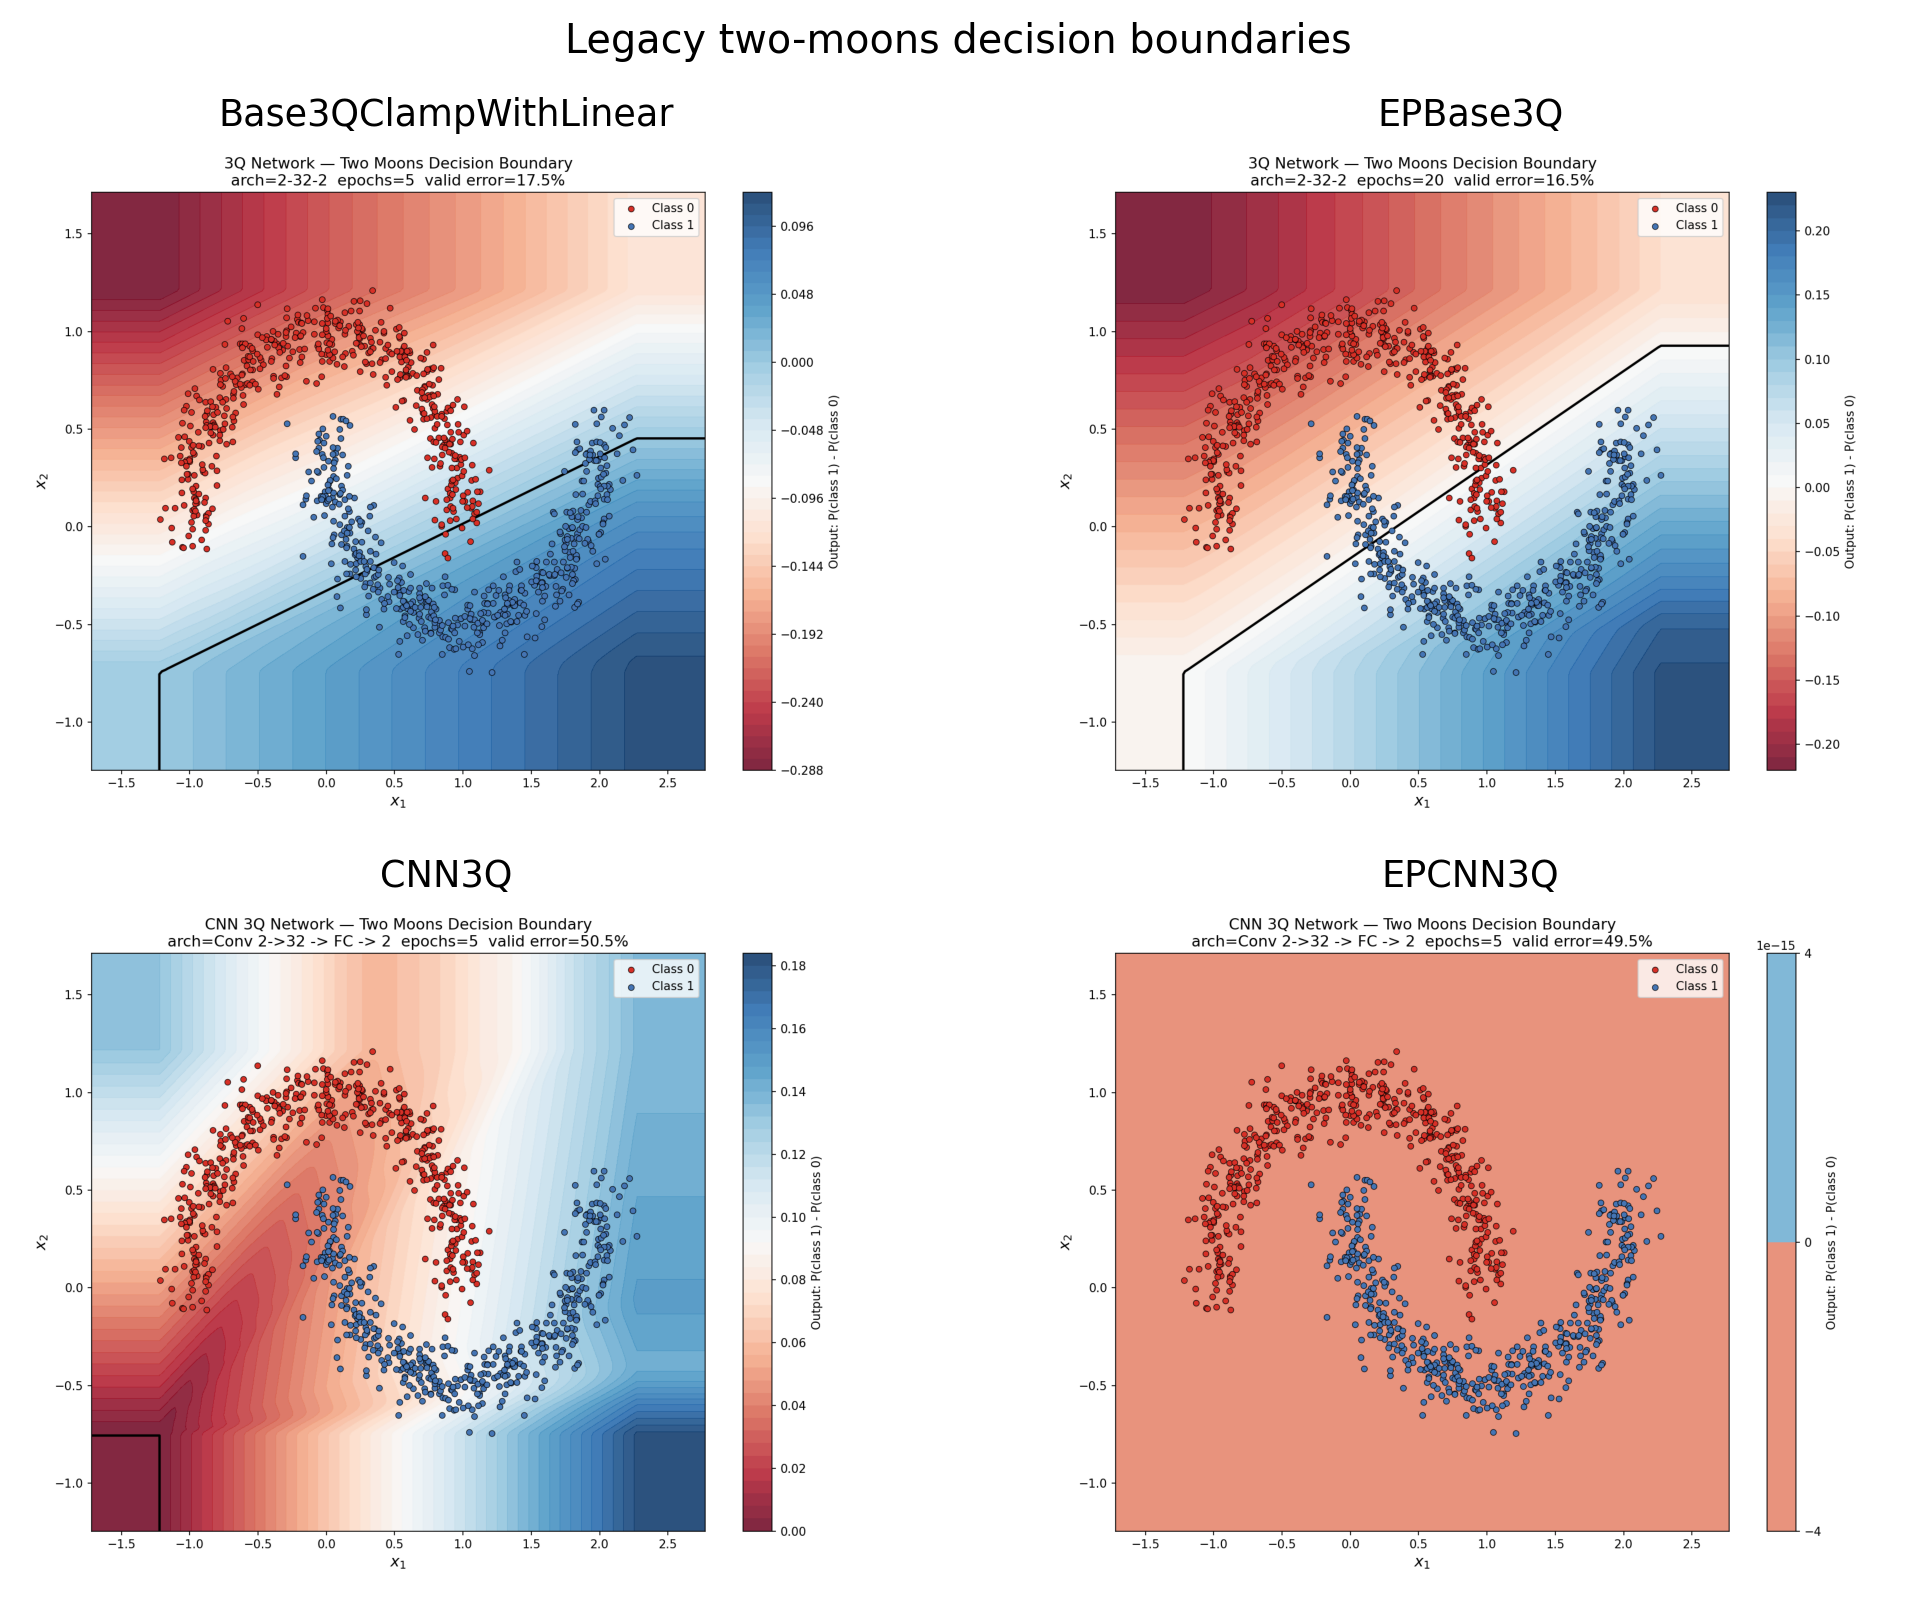
\includegraphics[width=0.94\linewidth]{fig11_legacy_cnn_decision_boundaries.png}
        \caption{legacy two-moons decision-boundary 图。CNNThreeQ/EPCNNThreeQ 是结构推广线索，但需要独立可比较 suite 验证。}
        \label{fig:cnn-legacy}
        \end{figure}

        \begin{table}[H]
        \centering
        \caption{MNIST small-budget screen 中 BP、ThreeQ、EPThreeQ、CNNThreeQ 的对照。该表用于说明短预算公共框架失败形态，不代表 legacy 完整预算结论。}
        \resizebox{\linewidth}{!}{%
        \begin{tabular}{llrrrr}
        \toprule
        variant & family & best acc. mean & final acc. mean & saturation & duration sec \\
        \midrule
        bp\_mlp\_tanh & bp\_mlp & 0.8886 & 0.8886 &  & 33.6811 \\
bp\_cnn & bp\_cnn & 0.8812 & 0.8812 &  & 33.4429 \\
epcnnthreeq\_ep & legacy\_conv & 0.1283 & 0.1283 &  & 38.5599 \\
cnnthreeq\_direct & legacy\_conv & 0.1241 & 0.1195 &  & 38.3474 \\
epthreeq\_cost\_w10 & threeq\_mlp & 0.0957 & 0.0957 & 0.4517 & 45.1293 \\
threeq\_direct\_cost\_w10 & threeq\_mlp & 0.0837 & 0.0837 & 0.3859 & 44.2015 \\
        \bottomrule
        \end{tabular}}
        \end{table}

        未来 CNNThreeQ 应建立独立 \texttt{experiments/cnn\_suite}：固定数据、seed、batch、推断步数、学习率和诊断指标，并记录 best/final error、state delta、rho 或替代谱指标、saturation、weight scale 和 runtime。更关键的是，卷积版本不应让所有像素 reconstruction 与分类项同权；应测试 patch/block energy、channel-wise normalization、pooling state 和高层 supervised nudging。

        \section{总体结论}

        \begin{enumerate}[leftmargin=2em]
        \item \textbf{ThreeQ inference 的理论与实验闭环已经较清楚。} $\rho(J)<1$ 是局部收敛的可观测充分条件；受控线性实验补足了 $\rho>1$ 的指数发散证据；训练压力测试说明大步更新可以跨越稳定边界。
        \item \textbf{基础 ThreeQ 能学习，但慢且敏感。} 原始 ThreeQ 不是无法学习 MNIST；问题在于 hard clipping、局部平均预测和 detach 使训练效率低，公共小预算设置会严重低估 legacy 架构。
        \item \textbf{EPThreeQ 是当前最稳的原始改进线。} EPBase3Q 在 10k/2k、15 epoch 上达到约 86.5\% accuracy，且训练中的 $\rho$ 保持在稳定区间。
        \item \textbf{DThreeQ 的 EP/CE-nudge 分支可行。} DThreeQ full-data restore-best 达到约 88.0\%，但 final 退化；Dplus 主规则未通过机制诊断，与 BP 方向不对齐，plusminus 已明确失败。
        \item \textbf{CNNThreeQ 是结构推广方向，不是当前性能结论。} Conv/ConvTranspose 结构自然对应严格转置共享，但仍需要独立 benchmark。
        \end{enumerate}

        \section{下一步研究方向}

        后续研究应优先推进五件事。第一，完整复现 legacy MNIST：把 EPBase3Q 的 \texttt{beta=1.0} 与 \texttt{weak\_steps=5} 扩展到 50k/10k、多 seed、保存 best checkpoint。第二，在公共框架逐项对齐 legacy hidden size、状态步数、$\epsilon$、$\beta$、初始化和训练预算，定位 small-budget 退化来源。第三，对 DThreeQ 使用 CE/softmax nudge、boundary-clamped input、layer-normalized energy 和 conservative schedule，目标是保住 full-data early best。第四，Dplus 方向需要结构性目标而非继续调尺度，例如 signed residual target、output-to-hidden residual injection 和带约束的 trainable layer gain。第五，CNNThreeQ 应从 energy 粒度重新设计，而不仅是把 MLP 边替换成卷积/反卷积。

        \section{局限性}

        本报告汇总的是截至当前仓库已有结果，其中部分 CNNThreeQ 图来自 legacy 脚本，不具备和 radas suite 相同的统计强度；DThreeQ full-data 结果显示 best checkpoint 和 final checkpoint 差异较大，因此不能只报告 selected accuracy；$\rho>1$ 的严格发散证据来自受控线性母模型，真实非线性 ThreeQ 中可能表现为振荡、停滞或饱和下的退化固定点，而不一定无界爆炸。论文写作中应保留这些边界条件。

        \end{document}
